% ************ Chapter 3 ************
\chapter{Planeamento do Projeto} 
\label{cap:3}
%Pretendia-se que fosse desenvolvido um sistema de informação completo para armazenar os registos feitos na fábrica. 

\section{Pré-projeto}
A primeira semana do projeto foi dedicada ao levantamento de requisitos. Existiam neste momento duas listas de requisitos distintas: requisitos absolutos\label{sym:REQUISITO_ABSOLUTO}, requisitos que a administração tinha uma noção exata do que pretendia e como pretendia, e requisitos indexados\label{sym:REQUISITO_INDEXADO}, que são requisitos sobre os quais a administração apenas consegue descrever o resultado que pretende.
Da lista de requisitos absolutos faziam parte os seguintes requisitos:
    \begin{itemize}
        \item A aplicação só poderia ser acessível da rede interna
        \item Uso de uma base de dados relacional
        \item Registo do horário de entrada e saída dos colaboradores
        \item Registo do peso e ponto de recolha de onde vinha a matéria prima
        \item Registo do peso de cera, metal e plástico de uma produção, bem como o colaborador associado.
        \item Registo do peso do produto final acabado
        \item Registo da saída de produto acabado e cliente a quem foi vendido
        \item Impressão de uma segunda via dos códigos de barras já impressos referente a uma recolha ou um produto acabado
        \item Incremento do peso de uma recolha efetuada anteriormente.
        \item Zona protegida por ID e Password para a consulta dos registos feitos
        \item Possibilidade de editar e apagar registos já feitos.
        \item Script de analise da coerência dos dados registados.
    \end{itemize}
Da lista de requisitos indexados faziam parte:
    \begin{itemize}
        \item Melhoria do design da base de dados
        \item A aplicação deveria ser acessível em dispositivos moveis e computadores
        \item Incremento do peso de uma recolha
    \end{itemize}


\section{Desindexação de requisitos}
Como forma de tornar os requisitos indexados em requisitos absolutos, durante a semana 1, foi feita um estudo completo da aplicação já existente, da sua base de dados e dos restantes requisitos indexados.
Concluída a analise foi desenvolvido um documento de proposta referente à plataforma e ferramentas a utilizar no desenvolvimento do sistema de informação. Esse documento cobria os seguintes aspetos:
\begin{itemize}
    \item \textbf{Tipo de Aplicação:} Aplicação Web, construida em PHP com framework Laravel e Javascript ou Aplicação Desktop em Java mais aplicação Android
    \item \textbf{Sistema operativo do Servidor:} Windows Server ou Ubuntu Server
    \item \textbf{Sistema de Gestão de Base de Dados:} Microsoft SQL Server ou MySQL
    \item \textbf{Tipo de plataforma:} Servidor virtual ou físico
\end{itemize}
O documento foi concluído com a proposta de se utilizar um servidor virtual com o Ubuntu para alojar a base de dados MySQL e a aplicação web.
A segunda reunião da semana foi exclusivamente para a discussão da proposta e das outras alternativas levantadas. A administração decidiu optar por uma aplicação web, mas demonstrou preferência pelo o sistema de gestão de base de dados Microsoft SQL Server. Aqui levantou-se a questão do Microsoft SQL Server poder ser usado num servidor com Ubuntu. Confirmada essa questão a administração decidiu usar um servidor físico com Ubuntu Server na versão 18.04.

Após esta reunião seguiu-se uma terceira reunião onde foi apresentada a proposta de estrutura da nova base de dados, descrita na figura \ref{fig:db_model old}.
\newpage
\begin{figure}[H] 
    \begin{center}
    % 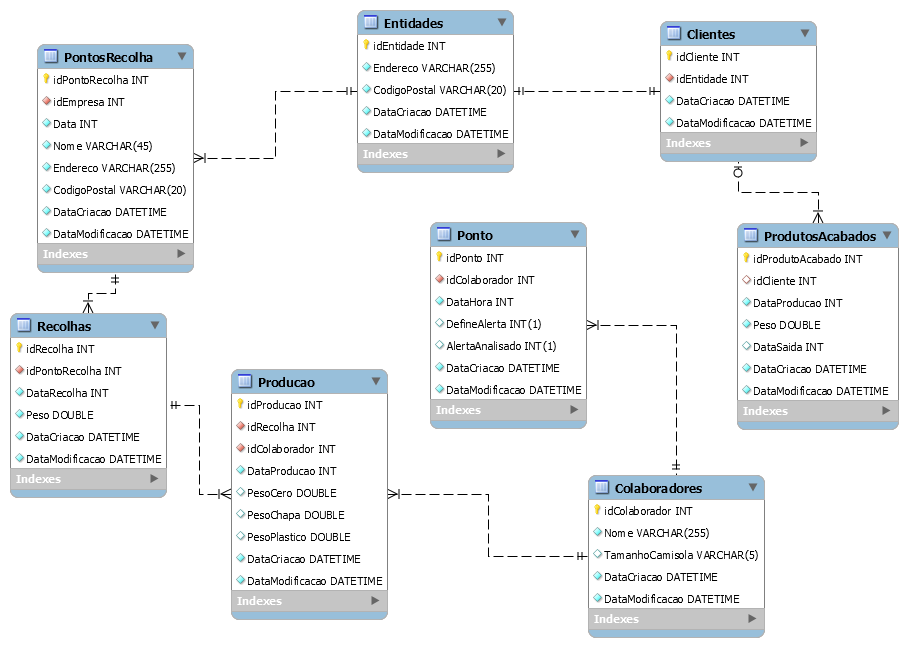
\includegraphics[width=\textwidth,keepaspectratio]{figuras/DB_Model/old.png}
    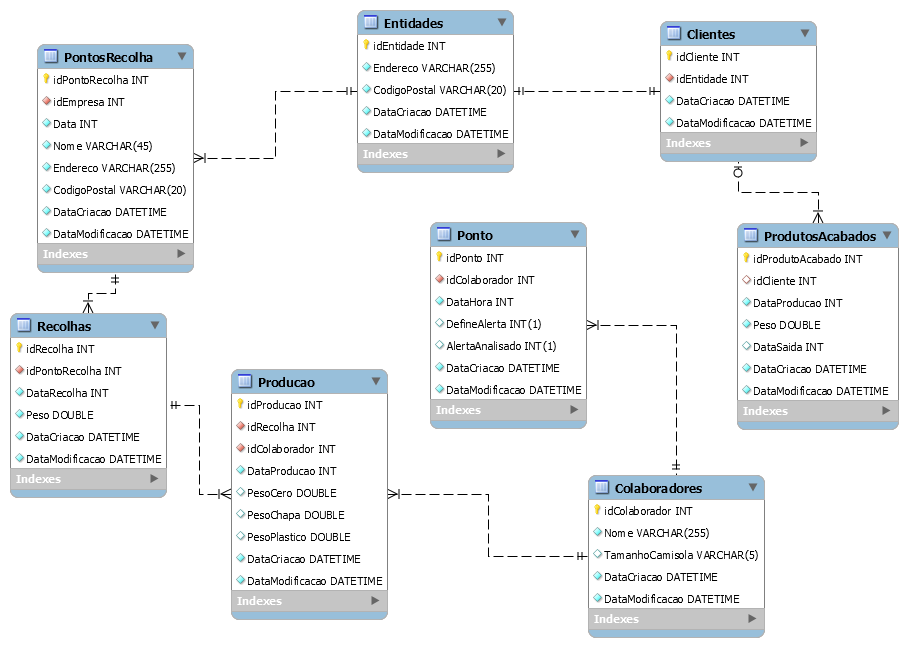
\includegraphics[width=\textwidth,keepaspectratio]{figuras/DB_Model/old.png}
    \caption{Primeiro modelo de base de dados apresentado}\label{fig:db_model old} 
    \end{center}
\end{figure}

Após a analise da administração, a reestruturação foi reprovada. Um dos motivos apresentados foi a separação dos tipos de fornecedores em tabelas distintas. De forma a manter uma maior compatibilidade com algumas ferramentas de analise já implementadas a administração optou por manter um campo na tabela pontos de recolha onde iria descrever o tipo de ponto de recolha. Durante esta reunião, discutiu-se ainda a funcionalidade de incremento do peso de uma recolha. Esta fazia-se necessária quando alguma recolha superasse a quantidade de material que era possível pesar de uma só vez. Para contornar este problema chegou-se à decisão de implementar um incrementador do peso de uma recolha com base no código já impresso.  Deveria ainda existir uma tabela extra na base de dados para registar o histórico de incrementos numa determinada recolha, de forma a auxiliar o operador, no momento do registo, a saber se aquele peso já tinha sido registado. Feitas as alterações indicadas pela administração, a estrutura da base de dados, descrita na figura \ref{fig:fig:db_model new}, foi aprovada.
\newpage
\begin{figure}[H] 
    \begin{center}
    % 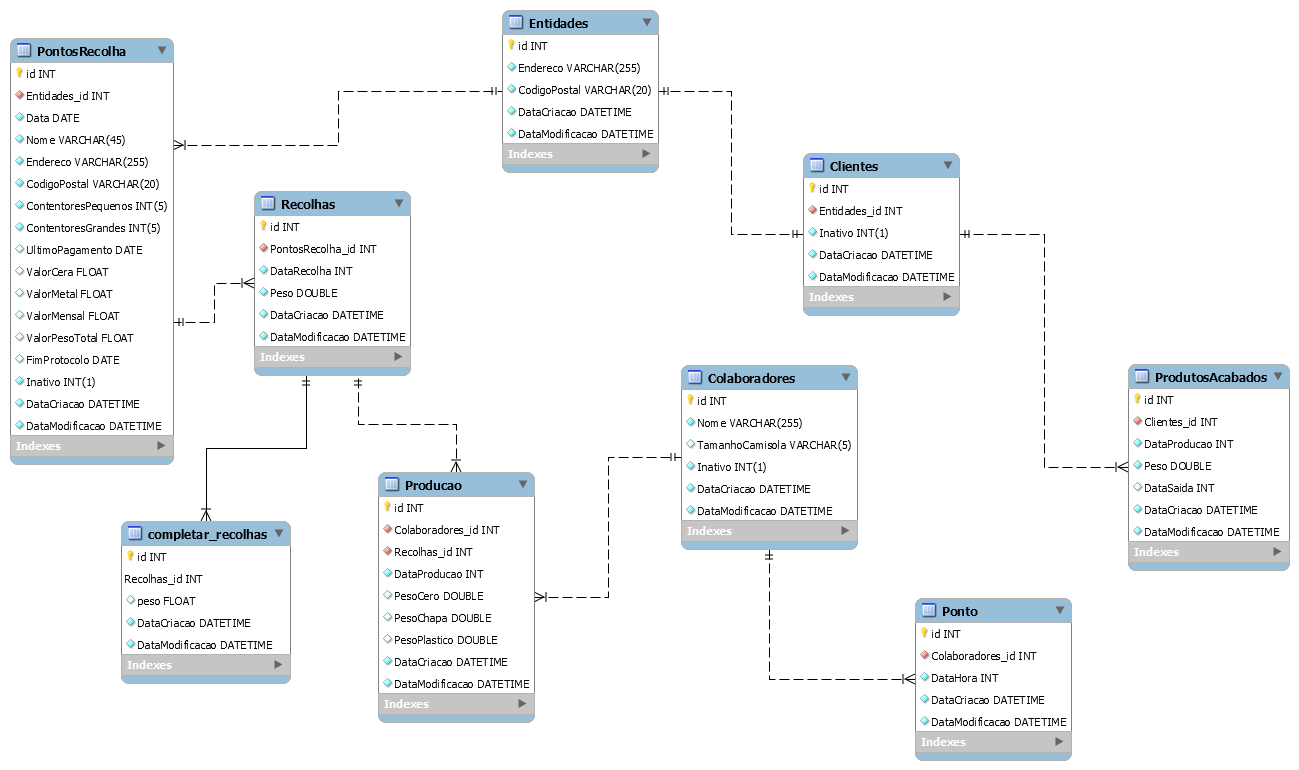
\includegraphics[width=\textwidth,keepaspectratio]{figuras/DB_Model/new.png}
    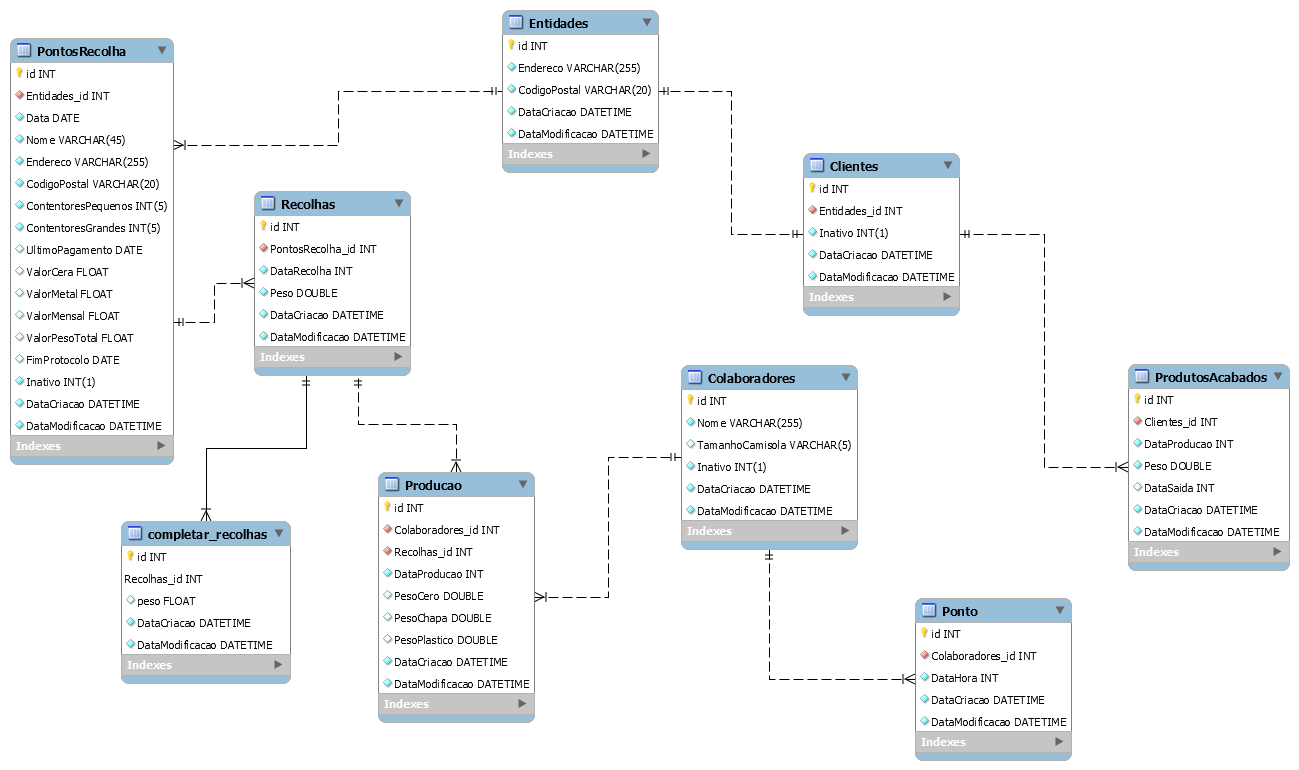
\includegraphics[width=\textwidth,keepaspectratio]{figuras/DB_Model/new.png}
    \caption{Segundo modelo de base de dados apresentado}\label{fig:fig:db_model new} 
    \end{center}
\end{figure}

Ao longo destas reuniões foram ainda levantados alguns novos requisitos para o projeto.
\newpage
\section{Lista final de requisitos}
Após as 4 reuniões de levantamento de requisitos, chegou-se à seguinte lista composta apenas por requisitos absolutos.
\begin{itemize}
    \item A aplicação só poderia ser acessível da rede interna
    \item Aplicação alojada num servidor físico com Ubuntu Server 18.04
    \item Aplicação WEB desenvolvida em PHP, com o framework Laravel, e em Javascrip.
    \item Uso de uma base de dados relacional, construida com o sistema de gestão de base de dados Microsoft SQL Server e a estrutura aprovada pela administração.
    \item A implementação teria de ser feita em duas fases, uma primeira onde se substituía totalmente a aplicação existente na fabrica, de modo a não parar o trabalho da fábrica ou ter de usar duas aplicações e uma segunda fase durante a qual as novas funcionalidades seriam aplicadas incrementalmente
    \item Devido à utilização de uma base de dados completamente reestruturada, antes da primeira implementação a aplicação teria de passar por uma fase de testes muito exigente para impedir erros que obrigassem ao uso da base de dados antiga.
    \item Registo do horário de entrada e saída dos colaboradores
    \item Registo do peso e ponto de recolha de onde vinha a matéria prima
    \item Possibilidade de incrementar o peso de uma recolha
    \item Se a recolha fosse iniciada com 0kg (zero quilogramas) é iniciado automaticamente o processo de incremento do peso da recolha que acabou de ser registada.
    \item Impressão de um código de barras com o ID gerado para a recolha inserida
    \item Registo do peso de cera, metal e plástico de uma produção, bem como o colaborador associado.
    \item Registo do peso do produto final acabado
    \item Impressão de um código de barras com o ID gerado para a produto final acabado
    \item Registo da saída de produto acabado e cliente a quem foi vendido
    \item Impressão de uma segunda via dos códigos de barras já impressos referente a uma recolha ou um produto acabado
    \item Incremento do peso de uma recolha efetuada anteriormente.
    \item Zona protegida por ID e Password para a consulta dos registos feitos
    \item As tabelas apresentadas na interface da aplicação teriam de ser capazes de refletir alterações na estrutura das tabelas da base de dados.
    \item Possibilidade de registar e apagar utilizadores na plataforma.
    \item Possibilidade de registar e apagar colaboradores.
    \item Possibilidade de registar e apagar Pontos de Recolha.
    \item Possibilidade de registar e apagar Clientes.
    \item Possibilidade de editar e apagar registos já feitos.
    \item Possibilidade de inserir/editar/apagar/executar comandos SQL personalizados.
    \item Script de analise da coerência dos dados registados.
\end{itemize}


\section{Metodologia de gestão de Projetos}
A metodologia de gestão de projetos escolhida foi o Scrum. As reuniões com o \textit{product owner}, que neste caso seria a administração, ficaram marcadas para a sexta feira ao fim do dia. Nestas reuniões seriam apresentados os desenvolvimentos da semana e definido o trabalho para a semana seguinte.
Sem prejuízo destas reuniões, diariamente havia uma reunião apenas com o supervisor da empresa como forma de ter informação mais atualizada.
Relativamente ao lançamento de novas versões para produção a metodologia foi diferente em dois momentos:
\begin{itemize}
    \item Antes da substituição da aplicação de fábrica em produção: Até que todas as funcionalidades da aplicação estivessem disponíveis, as indicações eram para não disponibilizar nenhuma versão.
    \item Após da substituição da aplicação de fábrica em produção: Após a aplicação de fábrica estar em produção, o lançamento de novas funções seria feito após a reunião com o supervisor, para que as funcionalidades ficassem disponíveis o mais rápido possível.
\end{itemize}

\section{Plataforma e ferramentas de desenvolvimento}
Para o desenvolvimento do projeto utilizou-se um conjunto alargado de ferramentas.
\subsection{Linguagens de Programação}
Tratando-se de uma aplicação web, optou-se pela linguagem de programação PHP em conjunto com o framework Laravel para o \textit{backend}\label{sym:BACKEND}, pela sua robustez e  maturidade\cite{Mansuri2018}.O \textit{frontend}\label{sym:FRONTEND} ficaria a cargo do Javascript com o framework jQuery e o \textit{template} AdminLTE.

\subsection{Base de dados}
Como definido nos requisitos, o Sistema de Gestão de Base de Dados escolhido foi o Microsoft SQL Server e a aplicação para gerir a base de dados foi o SQL Server Management Studio.

\subsection{Versionamento}
Para gerir as versões do código fonte, foi utilizado um repositório privado no GitHub, com duas \textit{banches}\label{sym:BRANCH}: master e release.
Na \textit{banches} master era colocado o código que ia sendo desenvolvido e na release era colocado o código testado e pronto a ir para produção.
Como cliente para este serviço foi utilizado o GitKraken.